\providecommand{\main}{..}
\documentclass[main.tex]{subfiles}

\begin{document}
\chapter{Acoustic Design}
In this chapter all aspects related to the acoustic and physical design of the speakers will be discussed.
\section{Cabinet Design}
\subsection{Driver Choice}
An important defining step in the early stage of speaker design is the choice of speaker drivers. 
This determines the type of speaker, the quality of the speaker, the size of the speaker, and the cost of the speaker.
Because of this careful consideration must be taken to make sure the selected drivers suit the specific application and are good enough quality.

The drivers chosen were the Visaton SC 10 N\cite{tweeter} for the tweeter, and the Tymphany GS-135F25AL02-04\cite{woofer} for the woofer.
The cost for these was £12.03 for the tweeter and £25.08, giving a total cost of £37.11 for the drivers of one speaker.
This is a very modest price for a hi-fi speaker, but that was part of our aim in designing the speakers.

The woofer was chosen as it was suitable for a sealed cabinet design, and gives a cabinet size in the range that we desire.
The specific discussion of why this driver is suitable is in \ref{woofercalcs}.
The tweeter was chosen as its frequency range crosses over significantly with that of the woofers, ensuring that the speaker will have good performance over the full output frequency range.
The frequency responses can be seen in figure \ref{fig:driverFreqResponse}.
\begin{figure}
    \centering
    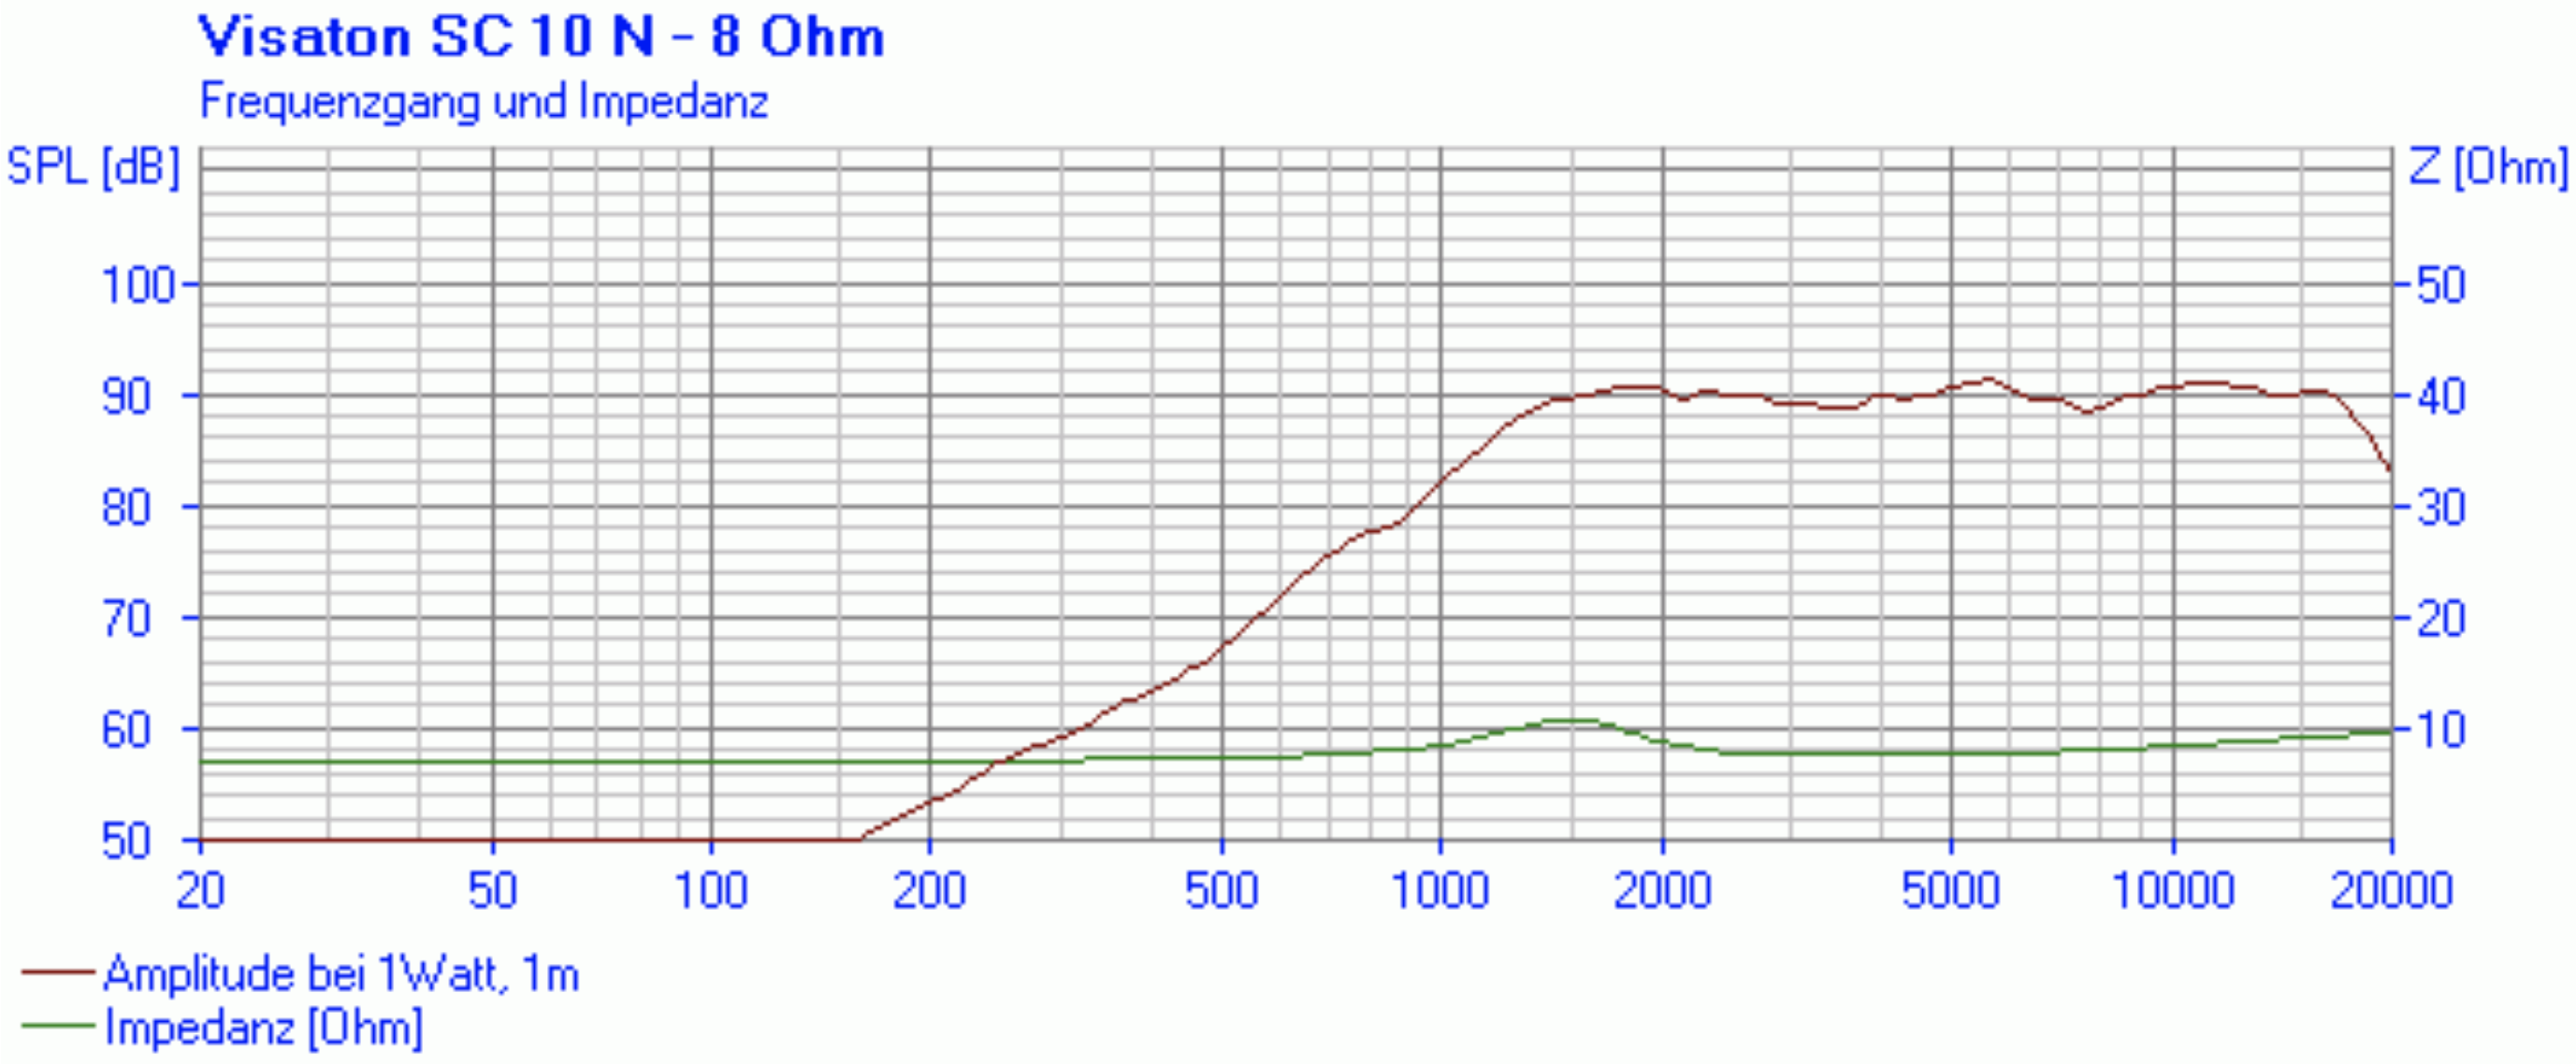
\includegraphics[width=0.9\textwidth]{figs/tweeter-response.png}
    
    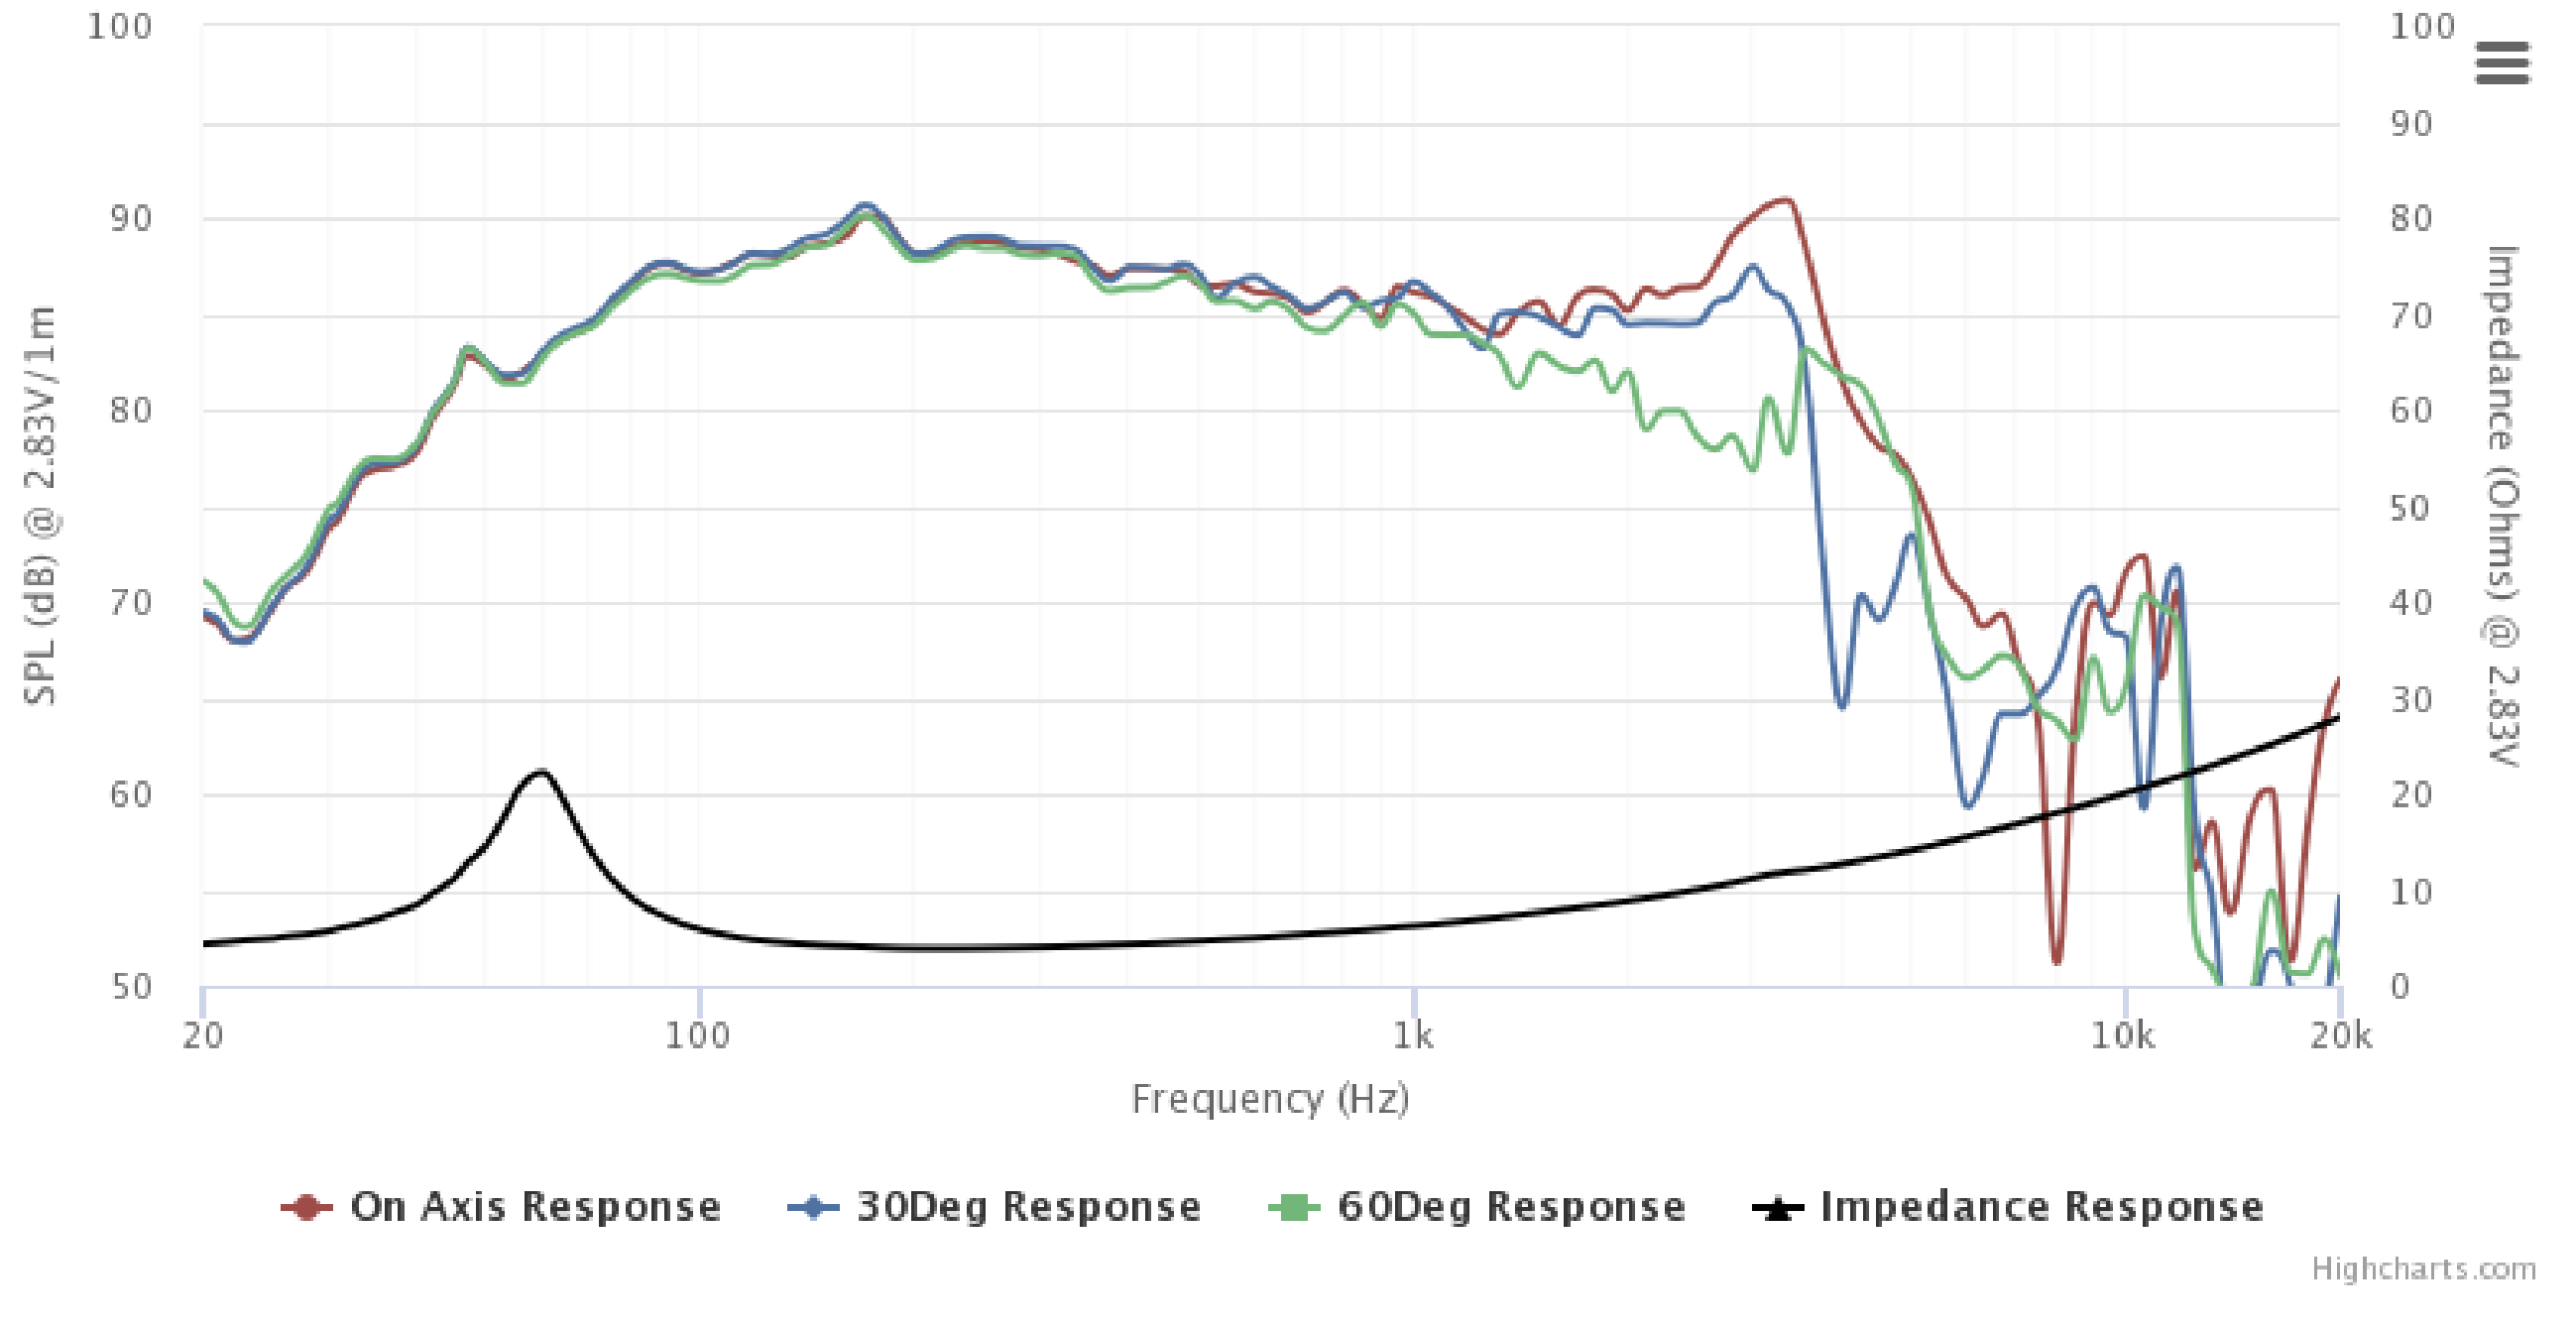
\includegraphics[width=0.9\textwidth]{figs/woofer-response.png}
    \caption{The frequency responses of the two selected drivers, as supplied from their datasheets.\cite{tweeter,woofer}}
    \label{fig:driverFreqResponse}
\end{figure}

\subsection{Woofer Calculations}
\label{woofercalcs}
Tweeters are totally enclosed devices and as such they can simply be mounted with no consideration having to be given to how or what is it is mounted on.
Woofers alternatively pose a greater complication as their performance is heavily determined by the physical enclosure it is mounted on.

The two main types of enclosure are sealed and ported enclosures.
Ported enclosures give better lower frequency response, but also results in higher volume cabinets for the same driver.
In addition, ported cabinets require much more precise construction and tuning, as the resonant frequency of the enclosure is extremely important to the performance.
While ported cabinets require precise tuning, the only important attribute of a sealed cabinet is its volume, which affects the actual system $Q_{tc}$.
This is a design choice, which is commonly chosen to be equal to $0.707$ in order to give maximal flatness.
A higher value of $Q_{tc}$ results in a peak resonance, while lower $Q_{tc}$ gives a steeper frequency roll off.
This can be seen in figure \ref{fig:qtcplot}.
In order to obtain a flat frequency roll off a value of 0.707 was used in this design.
\begin{figure}
    \centering
    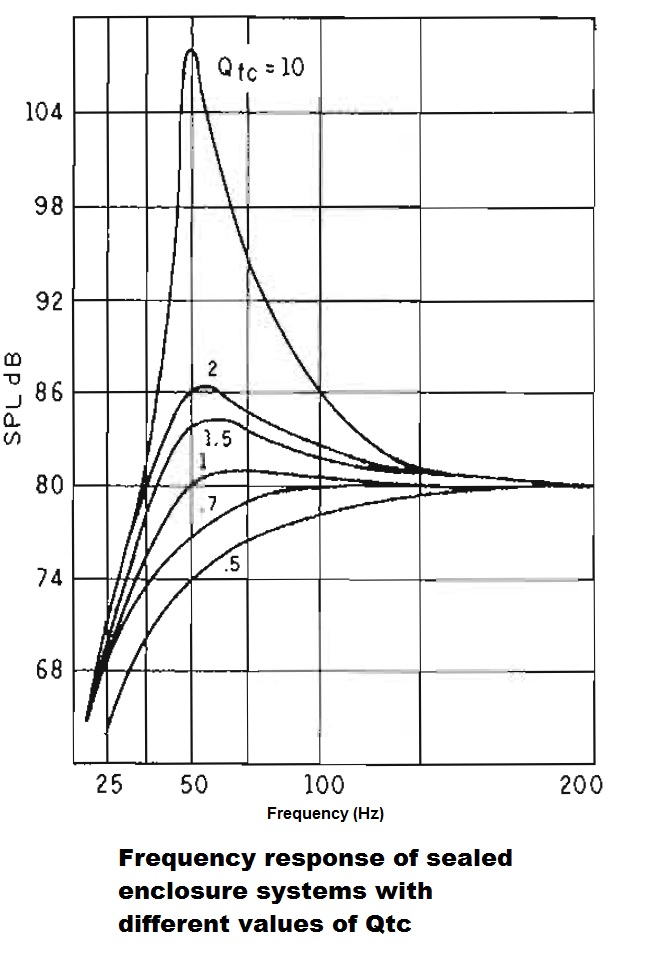
\includegraphics[width=0.5\textwidth]{figs/qtcResponsePlot.jpg}
    \caption{A plot showing the affect of $Q_{tc}$ on the frequency response of the system. Reproduced from \cite{qtcPlot}}
    \label{fig:qtcplot}
\end{figure}

Using the Thiele/Small\footnote{Thiele/Small parameters of speaker drivers are the parameters that } parameters from the data sheet of the woofer\cite{woofer}, the specific parameters of the selected driver can be calculated.

The first parameter to consider is the efficiency bandwidth product (EBP).
This determines whether the driver is suited for a sealed or ported enclosure, and is found to be:
\begin{equation}
    \mbox{EBP} = \frac{f_s}{Q_{es}} = 95.4
\end{equation}
where $f_s$ is the resonant frequency of the driver and $Q_{es}$ is the electrical Q of the driver at $f_s$.
A rough guide to use for EBP is that a driver with a value of 50 or below is recommended to be used with a sealed cabinet.
A woofer with EBP between 50 and 100 can be used for either.
This means that the driver is just on the outer range of acceptability for a sealed design, but it was the best performing for the price so it was chosen.

The internal volume of the enclosure can then be calculated using:
\begin{equation}
    V_b = \frac{V_{as}}{\left(\frac{Q_{tc}}{Q_{ts}}\right)^2-1}=\SI{6.49}{\liter}
\end{equation}
where $Q_{tc}=0.707$ as decided earlier, $V_{as}$ is the air volume equal to the compliance of the driver suspension and $Q_{ts}$ is the total system $Q$ at $f_s$.
These are obtained from the datasheet for the driver.

The frequency where the power dropped by the system is 3dB can also be found, which gives an indication of the lower frequency range of the total speaker:
\begin{equation}
    f_3 = \frac{Q_{tc}f_s}{Q_{ts}}\sqrt{\frac{\frac{1}{Q_{tc}^2}-2+\sqrt{\left(\frac{1}{Q_{tc}^2}-2\right)^2+4}}{2}}=\SI{78.68}{\hertz}
\end{equation}
This is a reasonable value for a speaker of the size that we are designing.
There are approximately two octaves of audible sound below this frequency, as \SI{20}{\hertz} is the lower limit of human hearing.
This is extremely respectable performance for a speaker of this size, and for this cost.
\subsection{Dimensions}
Now that the internal volume of the enclosure has been calculated, the dimensions of the speaker can now be decided.
The main consideration for the dimensions of the internal enclosure is to prevent the interference of standing wave resonances.
These occur when the sound waves from the woofer reflect and resonate with the walls of the speaker.
They become a real problem when the different surfaces resonate with the overtones of the other surfaces.
More complexly shaped cabinets can minimise this, but for a rectangular enclosure the aspect ratio which best minimises these overtone resonances is based on the golden ratio:
\begin{equation}
    \frac{1}{\phi}:1:\phi
\end{equation}
Using the previously calculated value for the volume of the box, this gives dimensions for the internal cavity as:
\begin{equation}
    \SI{300}{\milli\meter}\times\SI{186}{\milli\meter}\times\SI{115}{\milli\meter}
\end{equation}
These have been rounded to ease the construction of the box.

The woofer enclosure is the most significant part of the design acoustically, but as long as it is correct there is a lot of liberty to be taken with the rest of the design.
In this case, the back of the woofer cabinet is used as an internal wall within the full speaker cabinet.
The cabinet extends beyond the acoustic cabinet to contain another, smaller enclosure where the electronics and wireless system are to be placed.
In order to keep the symmetry of the design, the cabinet extends so that its base is a square.

The final considerations are the choice of material.
MDF is a material that is easy to work with and is a common material for DIY speaker building.
\SI{12}{\milli\metre} was assumed to be thick enough to fully dampen the 
\section{Construction and Manufacturing}

The enclosure was built from stock 12mm MDF and thus required various steps to assemble:

\begin{enumerate}
    \item A 4' x 8' 12mm MDF panel was quartered and cut to the size of the required plates using a jigsaw.
    \item Holes for the drivers in the faceplate were cut using the jigsaw, and screwholes drilled using a drill press.
    \item The enclosure was arranged in place and lightly bound with masking tape, then allowed to lay flat.
    \item A bead of PVA wood glue was spread across adjoining edges, and the enclosure taped back in place and clamped firmly.
    \item The glue was left overnight to set and the reinforcing tape and clamps removed.
    \item Seams were filled with a wood filler, left to dry, and the excess filler and sharp edges smoothed with 120 grit sandpaper
    \item Several coats of white MDF primer were applied and sanded until smooth.
    \item The desired design was masked onto the cabinets and several base white coats of acrylic spray paint applied.
    \item stripes were masked off and subsequent colours applied, allowing 10 minutes to dry between coats.
    \item All masking tape was removed and the speaker drivers bolted in place.
    \item The full enclosure was given several coats of a clear spray lacquer to protect the paint.
    \item The internal plate's position was marked, speaker wires were fed through, and it was glued in place.
    \item Holes were drilled to accommodate the panel mount volume buttons, power switch, and DC barrel jack.
    \item 12mm extensions for the tactile switches were 3D printed out of PLA and glued to the switch board
    \item The back panel was sanded to a tight friction fit onto the speaker enclosure and attached.
\end{enumerate}


\end{document}